\documentclass{article}
% Include all project wide packages here.
\usepackage{fullpage}
\usepackage{polyglossia}
\setmainlanguage{dutch}
\usepackage{csquotes}
\usepackage{graphicx}
\usepackage{epstopdf}
\usepackage{pdfpages}
\usepackage{caption}
\usepackage[list=true]{subcaption}
\usepackage{float}
%\usepackage{mathtools}
\usepackage{standalone}
\usepackage{import}
\usepackage{tocloft}
\usepackage{wrapfig}
\usepackage{authblk}
\usepackage{array}
\usepackage{booktabs}
\usepackage[toc,page,title,titletoc]{appendix}
\usepackage{xunicode}
\usepackage{amsmath}
\usepackage{fontspec}
\usepackage{unicode-math}
\usepackage[
    backend=bibtexu,
	texencoding=utf8,
bibencoding=utf8,
    style=ieee,
    sortlocale=nl_NL,
    language=auto
]{biblatex}
\usepackage{listings}
\newcommand{\includecode}[3][c]{\lstinputlisting[caption=#2, escapechar=, style=#1]{#3}}
\newcommand{\superscript}[1]{\ensuremath{^{\textrm{#1}}}}
\newcommand{\subscript}[1]{\ensuremath{_{\textrm{#1}}}}


\newcommand{\chapternumber}{\thechapter}
\renewcommand{\appendixname}{Bijlage}
\renewcommand{\appendixtocname}{Bijlagen}
\renewcommand{\appendixpagename}{Bijlagen}

\usepackage[hidelinks]{hyperref} %<--------ALTIJD ALS LAATSTE

\renewcommand{\familydefault}{\sfdefault}

\setmainfont[Ligatures=TeX]{Myriad Pro}
\setmathfont{Asana Math}
\setmonofont{Lucida Console}

\usepackage{titlesec, blindtext, color}
\definecolor{gray75}{gray}{0.75}
\newcommand{\hsp}{\hspace{20pt}}
\titleformat{\chapter}[hang]{\Huge\bfseries}{\chapternumber\hsp\textcolor{gray75}{|}\hsp}{0pt}{\Huge\bfseries}
\renewcommand{\familydefault}{\sfdefault}
\renewcommand{\arraystretch}{1.2}
\setlength\parindent{0pt}

%For code listings
\definecolor{black}{rgb}{0,0,0}
\definecolor{browntags}{rgb}{0.65,0.1,0.1}
\definecolor{bluestrings}{rgb}{0,0,1}
\definecolor{graycomments}{rgb}{0.4,0.4,0.4}
\definecolor{redkeywords}{rgb}{1,0,0}
\definecolor{bluekeywords}{rgb}{0.13,0.13,0.8}
\definecolor{greencomments}{rgb}{0,0.5,0}
\definecolor{redstrings}{rgb}{0.9,0,0}
\definecolor{purpleidentifiers}{rgb}{0.01,0,0.01}


\lstdefinestyle{csharp}{
language=[Sharp]C,
showspaces=false,
showtabs=false,
breaklines=true,
showstringspaces=false,
breakatwhitespace=true,
escapeinside={(*@}{@*)},
columns=fullflexible,
commentstyle=\color{greencomments},
keywordstyle=\color{bluekeywords}\bfseries,
stringstyle=\color{redstrings},
identifierstyle=\color{purpleidentifiers},
basicstyle=\ttfamily\small}

\lstdefinestyle{c}{
language=C,
showspaces=false,
showtabs=false,
breaklines=true,
showstringspaces=false,
breakatwhitespace=true,
escapeinside={(*@}{@*)},
columns=fullflexible,
commentstyle=\color{greencomments},
keywordstyle=\color{bluekeywords}\bfseries,
stringstyle=\color{bluestrings},
identifierstyle=\color{purpleidentifiers}
}

\lstdefinestyle{vhdl}{
language=VHDL,
showspaces=false,
showtabs=false,
breaklines=true,
showstringspaces=false,
breakatwhitespace=true,
escapeinside={(*@}{@*)},
columns=fullflexible,
commentstyle=\color{greencomments},
keywordstyle=\color{bluekeywords}\bfseries,
stringstyle=\color{redstrings},
identifierstyle=\color{purpleidentifiers}
}

\lstdefinestyle{xaml}{
language=XML,
showspaces=false,
showtabs=false,
breaklines=true,
showstringspaces=false,
breakatwhitespace=true,
escapeinside={(*@}{@*)},
columns=fullflexible,
commentstyle=\color{greencomments},
keywordstyle=\color{redkeywords},
stringstyle=\color{bluestrings},
tagstyle=\color{browntags},
morestring=[b]",
  morecomment=[s]{<?}{?>},
  morekeywords={xmlns,version,typex:AsyncRecords,x:Arguments,x:Boolean,x:Byte,x:Char,x:Class,x:ClassAttributes,x:ClassModifier,x:Code,x:ConnectionId,x:Decimal,x:Double,x:FactoryMethod,x:FieldModifier,x:Int16,x:Int32,x:Int64,x:Key,x:Members,x:Name,x:Object,x:Property,x:Shared,x:Single,x:String,x:Subclass,x:SynchronousMode,x:TimeSpan,x:TypeArguments,x:Uid,x:Uri,x:XData,Grid.Column,Grid.ColumnSpan,Click,ClipToBounds,Content,DropDownOpened,FontSize,Foreground,Header,Height,HorizontalAlignment,HorizontalContentAlignment,IsCancel,IsDefault,IsEnabled,IsSelected,Margin,MinHeight,MinWidth,Padding,SnapsToDevicePixels,Target,TextWrapping,Title,VerticalAlignment,VerticalContentAlignment,Width,WindowStartupLocation,Binding,Mode,OneWay,xmlns:x}
}

%defaults
\lstset{
basicstyle=\ttfamily\small,
extendedchars=false,
numbers=left,
numberstyle=\ttfamily\tiny,
stepnumber=1,
tabsize=4,
numbersep=5pt
}
\usepackage{verbatim}


\begin{document}
\subsection {Efficientie}
Het belangrijkst is wel het analyseren van de data. Hoe efficient is het circuit? Het circuit dat bij ons gemaakt is, was groot. De efficientie was in het begin hoog (90\%), maar dan kan het programma niet alle aansluitingen realiseren. Vervolgens moet je zelf een box tekenen, waarin je de grootte handmatig aangeeft. Daarbij werden efficienties tot 30\% behaald. Eerst kwamen efficienties van 3-5\% naar boven, maar na een aantal regels veranderd te hebben, behaalden we steeds tussen de 20 en 30 \%.  \newline \\
De vraag die bij opkomt bij een alu is of hij bij weinig bits efficienter is dan bij veel bits (het aantal bits input is immers onze parameter). Dat is getest. Het resultaat kun je afbeelden door het aantal bits uit te zetten tegen de verkregen efficientie. Op deze manier kun je analyse doen op de data die je binnen krijgt. Het resultaat hiervan staat in de grafiek in figuur \ref{a1}. De screenshots, de basis voor deze figuur, staan in bijlage \ref{c1}. 
\begin{figure} [h!]
\begin{center}
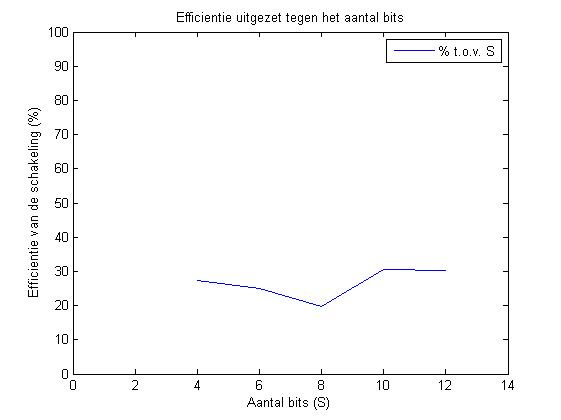
\includegraphics [scale = 0.5] {figures/efftot}
\caption{Grafiek van de efficientie: efficientie versus aantal bits}
\label{a1}
\end{center}
\end{figure}
Wat zegt dit plaatje nu? Ten eerste dat de efficientie niet hoog is. Dat is hierboven uitgelegd. Verder is te zien dat de efficientie niet toeneemt naarmate het aantal bits input kleiner is. Dat kan komen doordat je nu volstrekt willekeurig een box tekent om je layout heen waar je circuit hopelijk inpast. Als je een circuit zou nemen dat wel binnen de place\&route ruimte "past", dan kun je beter zeggen of de efficientie hoger is bij minder inputbits. 

\subsection{Grootte van het ciruit}
Verder is het opmerkelijk dat ons circuit onevenredig groot blijft wanneer het aantal bits afneemt. Dan blijven er errors verschijnen, niet in de synthese of compiler, maar in seadaly.  (waardoor je weer handmatig een box moet gaan tekenen) Hieruit kun je óf de conclusie trekken dat de alu een groot component is, omdat er zoveel operaties plaats moeten vinden, óf dat onze behaviour niet efficient is. Het zou interessant zijn om dit uit te zoeken, maar de tijd binnen het project laat dit niet toe. Als we onze alu bekijken, bestaan er geen aparte componenten (zoals een COMPONENT add of COMPONENT or), maar is alles 1 blok.  Als er meer tijd beschikbaar was zou nog uitgezocht kunnen worden of dit uitmaakt. Dan zou ook uitgezocht kunnen worden of de efficientie omhooggaat, wanneer voor elke operatie componenten gebruikt worden. 




\end{document}